%; whizzy chapter
% -initex iniptex -latex platex -format platex -bibtex jbibtex -fmt fmt
% 以上 whizzytex を使用する場合の設定。

%     Tokyo Debian Meeting resources
%     Copyright (C) 2006 Junichi Uekawa

%     This program is free software; you can redistribute it and/or modify
%     it under the terms of the GNU General Public License as published by
%     the Free Software Foundation; either version 2 of the License, or
%     (at your option) any later version.

%     This program is distributed in the hope that it will be useful,
%     but WITHOUT ANY WARRANTY; without even the implied warranty of
%     MERCHANTABILITY or FITNESS FOR A PARTICULAR PURPOSE.  See the
%     GNU General Public License for more details.

%     You should have received a copy of the GNU General Public License
%     along with this program; if not, write to the Free Software
%     Foundation, Inc., 51 Franklin St, Fifth Floor, Boston, MA  02110-1301 USA

%   Pdf作成手順
% dvipdfmx debianmeetingresume200509.dvi

%%ここからヘッダ開始。

\documentclass[mingoth,a4paper]{jsarticle}
\usepackage[dvipdfmx]{graphicx}
\usepackage{fancybox}
\usepackage{longtable}
\usepackage{ascmac}	% 囲み (screen,itembox)
\usepackage{fancyvrb}   % 囲み Verbatim のために必要
\usepackage[dvipdfmx]{hyperref}
\usepackage{url}

\AtBeginDvi{\special{pdf:tounicode EUC-UCS2}}

%% spacing の設定をする。外枠を減らす。
\setlength\headheight{0mm}
\setlength\topmargin{-20mm}
\setlength\headsep{0mm}
\setlength\topskip{3mm}
\setlength\maxdepth{4pt}
\setlength\columnsep{6mm}
\setlength\textheight{252mm}
\setlength\topmargin{-5mm}
\setlength\textwidth{170mm}
\setlength\oddsidemargin{-5mm}
\setlength\evensidemargin{-5mm}

% commandline環境を定義。画面入出力についてはcommandline環境
% で表記する
\newenvironment{commandline}%
{\VerbatimEnvironment
  \begin{Sbox}\begin{minipage}{15cm}\begin{fontsize}{7.3}{7.3} \begin{BVerbatim}}%
{\end{BVerbatim}\end{fontsize}\end{minipage}\end{Sbox}
  \setlength{\fboxsep}{8pt}\fbox{\TheSbox}}

%% 三択問題用の環境、DWNクイズで活用。
\newcounter{santakucounter}
\newcommand{\santaku}[4]{%
\addtocounter{santakucounter}{1}

\nopagebreak 問題\arabic{santakucounter}. 
#1\\
\nopagebreak□ A #2\\
\nopagebreak□ B #3\\
\nopagebreak□ C #4
\pagebreak[1]
\hspace{1cm}
\\

}

\newcommand{\emptyspace}{(\underline{\hspace{1cm}})}



\newcommand{\subsubsubsection}[1]{%
\vspace{1zw}{\bf #1}\\}


%% sectionをセンタリングする
\makeatletter
  \renewcommand{\section}{\@startsection{section}{1}{\z@}%
    {\Cvs \@plus.5\Cdp \@minus.2\Cdp}% 前アキ
    {.5\Cvs \@plus.3\Cdp}% 後アキ
    {\normalfont\Large\headfont\raggedright\centering}} % style
\makeatother

%% section の代わりの環境, ぐるぐるマークをつけるために、こちらを使ってく
%%  ださい。
\newcommand{\dancersection}[2]{%
\newpage
東京エリアDebian勉強会 2005
\hrule
\vspace{0.5mm}
\hrule
\hfill{}
\includegraphics[width=3cm]{image200502/openlogo-nd.eps}\\
\vspace{-4cm}
\begin{center}
  \section{#1}
\end{center}
\hfill{}#2\hspace{3cm}\space\\
\hrule
\hrule
\vspace{1cm}
}

%% for gotom
\newenvironment{gdescription}%  
{%
   \begin{list}{}% 見出し記号/直後の空白を調節
   {%
      \setlength{\itemindent}{0mm}
      \setlength{\leftmargin}{45mm}%  左のインデント
      \setlength{\rightmargin}{0zw}% 右のインデント
      \setlength{\labelsep}{4mm}%    黒丸と説明文の間
      \setlength{\labelwidth}{4cm}%  ラベルの幅
      \setlength{\itemsep}{0em}%     項目ごとの改行幅
      \setlength{\parsep}{0cm}%      段落での改行幅
      \setlength{\listparindent}{0cm}% 段落での一字下り
      \let\makelabel\gdescriptionlabel
   }
}{%
   \end{list}%
}
\newcommand*\gdescriptionlabel[1]{\hspace\labelsep\normalfont\bfseries #1}
%%

\begin{document}


\begin{titlepage}

% 毎月変更する部分
\title{
 第8回 東京エリア Debian 勉強会\\事前資料}
\date{2005年9月10日}
\author{Debian勉強会会場係 上川 純一\thanks{Debian Project Official Developer}} 
\maketitle
\thispagestyle{empty}
\end{titlepage}

\newpage
\tableofcontents

\dancersection{Introduction To Debian 勉強会}{上川 純一}

今月のDebian勉強会へようこそ。
これからDebianのあやしい世界に入るという方も、すでにどっぷりとつかってい
るという方も、月に一回Debianについて語りませんか?

目的として下記の二つを考えています。

\begin{itemize}
 \item メールではよみとれない、もしくはよみとってられないような情報を情
       報共有する場をつくる
 \item まとまっていないDebianを利用する際の情報をまとめて、ある程度の塊と
       して出してみる
\end{itemize}

また、東京にはLinuxの勉強会はたくさんありますので、Debianに限定した勉強
会にします。Linuxの基本的な利用方法などが知りたい方は、他でがんばってくださ
い。
Debianの勉強会ということで究極的には参加者全員がDebian Packageを
がりがりと作りながらスーパーハッカーになれるような姿を妄想しています。

Debianをこれからどうするという能動的な展開への土台としての空間を提供し、
情報の共有をしたい、というのが目的です。
次回は違うこと言ってるかもしれませんが、御容赦を。

\subsection{講師紹介}

\begin{itemize}
 \item{鵜飼さん} Debian JP のサーバたちにとってなくてはならない存在です。
 \item{やまねさん} DebianJPのウェブページに改革をもたらそうとしています。
 \item{上川 純一} 宴会の幹事です。
\end{itemize}

\subsection{事前課題紹介}

今回の事前課題は
「debconfをつかっていて答えるのにこまった質問」
というタイトルで200-800文字程度の文章を書いてください。
というものでした。
その課題に対して下記の内容を提出いただきました。

\subsubsection{澤田さん}

答えるのにこまった質問、最近一番こまったのはflexのバージョンが上がるとき
に「POSIX準拠じゃなくなるけどいいかい?いやならflex-old入れてね」という
質問だ。この質問はいけていない。何がいけていないかというと

* デフォルトがfalseな点

* falseと答えるとexit 1する点

の2点だ。exit 1するのでインストールエラーになる。エラーと言われるのでど
きどきする人が多いのではないだろうか。特にwoodyからsargeに上げようとして
はまった人が多いと思われる。いや、私のことですが何か?

mpichとlamみたいにflexとflex-oldを別々の場所にインストールして選んだ回答
に応じてalternativesを設定とかしてくれるとうれしい気がする。

falseと答えてインストール失敗した後、普通にapt-get install flex-oldでき
るのか?と試そうとするがfalseと答えてるのにインストールされてしまう。何
でだ?


\subsubsection{岡島さん}

簡単にDebian歴を紹介しますと、
Debianをはじめた原因の一つは、RedhatのFedora移行の混乱に嫌気がさしたことであって、
ようは始めたのは最近ですし、
さらに、依然として本業のほうは、顧客の意向もあってRedhatなので、
結論としては私のDebian経験は非常に乏しく、ようは単なる初心者なのですが、
一通り技術はわかるが、しかしDebianは初心者、という観点からの
コミュニティに対する貢献、というのもあるかと。

で、Debianの印象ですが、
「上手くいくときはいいのだが、いかないときに困る」、
というのが印象ですね。これは、apt-get 特有の問題ではなく、自動化を進めれば
どんなものにも当てはまることですが。

で、お題の「Debconfで困った質問」ですが、特にありません。
デフォルトで何も考えずインストールしますが、それで特段問題になったことはないですね。
これは、Debianのデフォルトの選択が結構賢い、ということでもあるのでしょうが。

が、しかし、パブロフの犬状態で反射的に「いえーす、イエース」と答えてしまう
インストールに不安があるのは事実ですし、それじゃあ商売にならないというのはもっといえます。

結論なんですが、出題者の鵜飼さんは、多分、勝手な推測ですが、もっと質問文をわかりやすく、、、
とかお考えなんだと思いますが、そんなことより、以下の3つのほうが歓迎されると思います。
どうせ、いくら質問文をわかりやすくしても、ほとんどの利用者は、
本能的に「イエース、イエース、イエーーーース」の連打でしょうし、
そもそも、それで使えなければ結局使えないですね。

1、Roll back, Snapshot, Checkpoint, Undo

ようは同じことなんですが、
単に、apt-get remove とかを、、、というのではなく、
もう、ファイルシステムレイヤーで、もろスナップショットや undo がほしいです。
まあ、これは、Debian の問題ではなく Linux の問題でもあるのですが、
Debian のように、システム領域にばりばり勝手なことをしていく
(と、Debianを知らない人が思い込みやすい)
システムにおいては、より重要かと。
それ以外の理由においても、この手の機能がLinuxに実装されると、
システム管理上の利点は非常に大きいので、なんとかならないか、といろいろ
個人的にも研究しているのですが、なかなか難しいです。

2、過去のDebを!

個人的な印象では、Debianは、常に勝手に最新のDebが入ってしまい、
それ以外の選択がない、という印象です。
Pinning とか、やり方はあるみたいですが、なんかよくわからない。
そのくせ、必ずしも最新バージョンが安定しているとは限らない。
Stableブランチでもそうなんですから、Sidならもっと。
さらに、勝手にアップグレードされたパッケージが不安定だった日には、途方にくれます。
どうやって戻すんですかね、これ。
というか、いま、Debootstrapで遊んでるのですが、
ことごとくすべてのブランチで不安定なのは、私の日ごろの素行のせいですかね。
当然、Pbuilderもコケます。
解決策ですが、どうも鵜飼さんがある程度やってるみたいですが、
ようは、過去のDebを保存しているアーカイブはないの?ということです。
それをつかって手軽にロールバックできるだけで、ずいぶんDebian の印象は違うでしょう。

3、インストールログを。

そんなの、とっくの昔にもうあるよ、とかいわれそうですが、
なにをシステム管理者がやったか、をきっちりログにしてもらえるとうれしいです。
Debconfの質問一つとっても、何にどう答えたか、次の管理者がすぐわかる。
さらに、何にどう答えたか、レポートにして顧客に送れる。そんなんだといいですね。

\subsubsection{中島さん} 
質問されても読まないから困らないらないと思う。それにたいして選択に数ないと思
うので適当に打っていけば、だいたい決まってくるのだから数打てば当たるわけで、ぜ
んぜん困らないと思う。困るはずがないと思う。 しかし困らないけれど、もしも困っ
たときのために、質問の内容と答えをノートに書いておくというのがいいと思う。これ
で万全だ。ノートに書いておけば、これで適当に打っても大丈夫だ。これで良いと思う
。 なんか間違っても大した支障はないと思うから適当に打っていけばいい。

\subsubsection{武藤さん}

メモするものが手元にないときに「 ○○ が変わったので、インストールが終わっ
たあとに ○○ を ○○ にしてそれから ○○ してください」という注意書きだけ出てく
るのが一番困るかな。

ほかは「debconfで困る点」になっちゃうけど、優先順位が適切に設定されて
いなくてhighでも質問攻めだったり、逆にhighだと重要な質問をしなかったり
(XFree86のキーボード設定とか)とか。あと、「戻る」をdialogベースでもで
きないかなぁ。

\subsubsection{小林儀匡さん}

debconfを使っていて答えるのに困った質問は色々とありましたが、
あまりに多くて思い出せないので具体的には挙げません。
代わりに、それに纏わることを書くことにします。

debconfを使っていて答えるのに困る質問はスキルの向上に伴いかなり減りましたが、
初めてインストールしたときにはやはり多かったです。
質問内容が分からず、
適当にデフォルトの答えで済ませてその場をしのぎました。
本当はそういったものは逐一手でメモをとっておいて後で再設定するべきなのでしょうが、
かなり多かった上に、
ディスプレイに表示された質問を紙にメモするという作業の空しさ (?) のため、
途中からは閾値を上げ、
多くの質問は分からなくてもメモせずにスルーしてしまいました。

自分と同様の思いをしている人が多いのか少ないのか分かりませんが、
debconf で出た質問の一覧、
あるいはせめて debconf で質問をしたパッケージの一覧が、
APT を使った一連のパッケージインストール作業の最後に表示されたらよいのに、
と感じています。
質問だけでなく、
「インストール後には〜を読むように」という注意喚起のメッセージも、
どうせなら、インストールプロセス中に表示するのではなく、
最後に表示させたほうが効果的でしょう。
パッケージインストール作業の最後に表示させずとも、
何らかのファイルに一覧を書き出すのも効果的かと思います。

\subsubsection{えとーさん}

ほとんど。
ちょっと試してみるかな?と思いinstallしてみたらいろいろ質問が
出てしまう、しかし、ちょっと試してみようかな。であって事前に
なにも調べずに入れてみることがほとんどなので、その際に聞かれても
答えられない。
特に用語が解らない場合などにはなにを聞かれてるのか解らない。
なので、debconfはdpkg-reconfigureしてから使うもの。っていうイメージ。
debconfの設定をエクスポート、インポートできる仕組みが簡単に使えると、
バックアップやdpkg-setselectionsとの合せ技ができていいのかなぁと思った。
\footnote{提出が〆切すぎていたので、印刷にはまにあい
   ませんでした}

\subsubsection{上川}

debconfの使い方がよくわかっていなくて、先日gotomさんにいわれるまで、質問
にキャンセルという選択肢があるのに気づいていませんでした。
問題答えるのに困るものがあるのと、好ましくない答えをするとインストールエ
ラーになってしまうパッケージがあるのが困り物です。

debconfで質問されてもほぼデフォルトにしています。
で、デフォルトでは動かないパッケージがあるといかりくるってバグをファイルしま
す。

%%% trivia quiz
\dancersection{Debian Weekly News trivia quiz}{上川 純一}

ところで、Debian Weekly News (DWN)は読んでいますか?
Debian 界隈でおきていることについて書いているDebian Weekly News.
毎回読んでいるといろいろと分かって来ますが、一人で読んでいても、解説が少
ないので、
意味がわからないところもあるかも知れません。みんなでDWNを読んでみましょう。

漫然と読むだけではおもしろくないので、DWNの記事から出題した以下の質問にこたえてみてください。
後で内容は解説します。

\subsection{2005年32号}
2005年8月9日です。

 \santaku{あるパッケージをアップロードした場合のdebianに与えるリスクを計
 算する方法が欲しいというリクエストに対して出て来た、
 現在どのパッケージがいちばんtestingに影響しているというのを調査するには}
 {グーグルで検索する}{\url{http://bjorn.haxx.se/debian/stalls.html} にある どのパッケージがどれ
 くらいのパッケージのtesting入りを邪魔しているかというページを見る}{ls
 -l / }
 \santaku{GNUStepで問題なのは何か}{FHSに全く準拠していなく、GNUStepをそ
 のままでFHSに準拠させるのは難しい。}{使いにくい}{動かない}
 \santaku{Ian Jacksonは、「Debian」 Core Consortiumについて何を宣言した
 か}{我々がDebianをのっとった}{Debianは使えない}{Debian Core Consortiumという名前は正式名称ではないので問題無い}
 \santaku{MySQL 4.0から4.1への移行についてどういうことが議論されたか}{libmysqlclient
 の移行のためにバグをファイルするのは、今はgcc 4.0の移行中なため、避けて
 欲しい。}{MySQLはもうすてよう}{PySQLに名前が変わりました}
 \santaku{Andrews Barthはgnome2.10をetchにいれよう、testingに入れるため
 にアップロードをしばら
 くひかえよう、とかけごえをかけましたが、出た反論が}{gnome2.10なんで誰も
 つかっていない}{Nathanael Nerode
 さんが言うには、xorgの移行によってブロックされてしまっているのでしばら
 くは無理 }{testingなんて存在しません}
 \santaku{Helen Faulknerさんが作成したメーリングリストは}{debian-science
 メーリングリスト}{debian-helen メーリングリスト}{ debian-faulknerメーリ
 ングリスト}
 \santaku{xorg6.9についてDavid Nusinowが報告したのは }{quiltベースのパッ
 チシステムに移行したおかげで以前までは数週間かかっていたパッチの移行が
 3-4日しかかからなくなりました。}{画面表示のいろあいが変わりました}{高速
 化しました}

\subsection{2005年33号}
2005年8月16日です。
 \santaku{Debianの12回目の誕生日はいつか}{2005年8月16日}{2006
 年8月16日}{2005年4月1日}
 \santaku{RCバグの影響でtestingからパッケージを削除される場合がある。そ
 の場合にどうしたらtestingにパッケージが戻るか}{リリースマネージャに賄賂
 をおくる}{リリースマネージャを人質にとる}{RCバグを全部修正する。}
 \santaku{カーネルのソースパッケージはlinux-source-2.6.12になっており、
 ソースの入ったバイナリパッケージはlinux-2.6になった。その理由は}{ピリオ
 ドの消費を節約するため}{ユーザを混乱させるため}{古
 いバージョンをアーカイブ内に維持しつつユーザのアップグレードを簡単にするため}
 \santaku{Debianメンテナはバグを上流に報告する義務がある、という点に関し
 て、Eric Dorlandが反論した理由は}{firefoxパッケージには300くらいのバグ
 が現在openされており、上流にフォワードするという作業だけで時間が無駄に
 とられてしまう。}{BTSなんか見てない}{自分では使っていないので使っている
 人が報告してほしい}
 \santaku{Joerg Jaspertが発表した、Debian Developer の追放の規則によると}
 {追放期間は一年間で、保釈金を支払うともどってこれる}
 {DPLのわるぐちを言ったDebian Developerは追放できる}{一旦追放されてもNMプロセスを経てDebian Developerにもどってこれる}
 \santaku{LinuxFundがDebianに対して実施すると発表したのは}{月 $500の
 資金提供を1年間実施する。}{Debian DVDを売る}{Debianを使う}
 \santaku{Hanna WallachがDebian Womenの現状について懸念を示した内容とし
 ては}{Debian Projectをのっとるためにはもっと高速にDebian Womenプロジェ
 クトが成長する必要がある}{Debian Womenという名前は性差別なのでDebian
 people と呼ぶべきだ}{女性のために簡単に入れるdebian-womenという新しいコミュニティー
 をつくるのが目標ではなく、Debian Developerに参加するための援助をしてい
 くのが目標なのでそれを忘れないように}
 \santaku{Andrews Schuldei が求めたのは}{Debian Developerたちが集まって
 作業するのと効率がよい場合もあるので、できる場所などの寄付}{個人的な利
 益}{世界人口の半分がDebian Developerになること}
 \santaku{Torsten Landschoff が提案したのは、共有ライブラリパッケージの
 SONAMEが変わっただけのような場合に関しては自動でftp-masterがACCEPTする
 仕組みだが、その仕組みに対しての反論は}{Joerg Jaspert曰く、空のパッケー
 ジがつい最近アップロードされていたので、そういう間違いが検出できるのは
 重要だ。}{Joerg Jaspert曰く、ftp-masterの権限を弱めるような実装はありえ
 ない}{Joerg Jaspert曰く、その実装の詳細な部分が気に入らない}
 \santaku{Gutenprintがunstableにリリースされた。以前はなんという名前だったか}{gimp-print}{gnome-print}{kde-print}%gimp-print

\subsection{2005年34号}
2005年8月23日です。
 \santaku{DCCに関して、Debian商標についての決定権を委任されたのは }{Don
 Armstrong}{Andreas Schuldei}{Branden Robinson}
 \santaku{gotom さんがglibcについて宣言したのは}{カーネル2.4しか動かない
 システムではコンパイルできないぞ。}{ドアストップアーキテクチャについて
 は、サポートはしない}{よくこわれるのでインストールしないでください。}
 \santaku{Steve Langasekによると、woodyからsargeの間のための移行パッケー
 ジというのは}{必要なので永遠に残す}{途中
 のリリースを省略したアップグレードはサポートしないので、woodyからsarge
 への移行専用のパッケージはunstableでは削除するべき}
 {バグが多いので対応してほしい}
 \santaku{Ramakrishnan Muthukrishnan さんと Ganesan Rajagopal があつく
 Debianについて語ったイベントは}{インドで実施したDebian Conference
 India}{日本で開催したDebian Conference}{中国で実施したDebian Asia Miniconf}
 \santaku{woodyにしかない古いバグをクローズするのはどうしたらよいか}
 {「君の事はずっと嫌いだった」と書いたメールをそのバグに対しておくりつけ
 る}{どのバージョンで問題が解決したのか、という情報をBTSに記録する}
 {woodyタグを付ける}
 \santaku{Lars が piupartsで実施してみたらどうなったか}{たくさんバグがみ
 つかった}{Debianは完全であることが立証された}{piuparts自身が動かなかった}
 \santaku{バグ報告にGPG鍵認証を要求する話についてどういう意見が出たか}{Debian Developer以
 外でもできるようにはすくなくともしてほしい}{バグ報告は高尚な行為なので
 Debian Developer以外は実施してはならない}{GPGより違う認証プロトコルを使
 おう}
 \santaku{BTSのLDAPゲートウェイはどうなったか。}{masterのポート10101にて稼働
 再開した}{止まったまま}{使えないのでステ}
\subsection{2005年35号}
2005年8月30日です。
 \santaku{Joerg Jaspertさんが発表したNEWキューでREJECTされる要因は}
 {DEB\underline{ }AUTO\underline{ }UPDATE\underline{ }DEBIAN\underline{
 }CONTROLを使っているCDBSのパッケージは拒否}{パッケージ名がglibc}{メンテ
 ナ名がkmuto@debian.org}
 \santaku{Debian GNU/kFreeBSDでは、Debian mainの何\%のパッケージが利用可
 能か}{81.69\%}{15\%}{3\%}
 \santaku{Andreas Barthさんがライブラリについて要求したのは}{すでに移行
 が多数並行しすぎているため、ライブラリのSONAMEの変更などは発生させない
 でほしい。}{ライブラリは全部static linkに変更すること}{
 ライブラリはすべてデバッグ情報を残す事}
 \santaku{バグ報告の影響をうけているユーザが投票することで、
重要度をトラッキングするランキングを実施しようという意見に対して、現在す
 ぐにでもできそうな方法は何か}{バグに最後に活動した日付によってランキン
 グを付ける}{
 ずBTSと Popularity Contestを連携させる}{電波によって影響度を推察}
 \santaku{POSIX ShellとしてPOSHを利用してスクリプトの試験を実施すること
 に対しての反論は?}{busyboxのシェルですらそれよりも機能があるため、実質
 的な利益が無い}{poshはつかえない}{posh はバグだらけだ}
 \santaku{Mozillaについてセキュリティーフィックスとして新しい上流バージョ
 ンを利用することに関しての理由は}
 {めんどくさい}{上流がそれじゃないと嫌だというから}
{Ubuntu向けにMartin Pittがセキュリティーフィックスのバックポートを
 けっこうな時間をさいて実施してみたが、難しかった}
 \santaku{Yaroslav Halchenko が十分なAMの人数がいるのに100日以上かかって
 いるのはNMプロセスが忍耐力を試験しているのではないか、というコメントを
 した際のMarc Brockschmidt の回答は}{陰謀なので気づかないでください}{
忍耐力を計測しているのにきづいちゃった?}{そんなことはなく、今一番活発な
 AMであるMarcとJoergは担当しているNMの数を減らそうとしている最中なので、AMが増え
 るのは好ましい}
 \santaku{Joey hess が debconfに依存しているけどdebconf-2.0に依存してい
 ないパッケージをなくしたいのは}
 {cdebconfに移行できるため}{debconf2.0の機能だけにしたいから}{debconfの
 バージョンを新しくしたいから}
 \santaku{lists.debian.orgにあるウェブ経由でのメールインタフェースで
メーリングリストのスパムを報告するリンクは何をするものか}{メーリングリス
 トにスパムを投げる}{メーリングリストにスパムが来てますというメールをメー
 リングリストの参加者にランダムに投げる}
 {実はまだ統
 計情報を集めているだけで何をするというものでもない}
 \santaku{ビルドするのにnon-freeなシステムが必要なパッケージはDFSG-Freeか}
 {DFSG-freeでもビルドするのにnon-freeなものが必要ならDFSG-Freeとは言えな
 い}{パッケージ自身のソースがフリーならフリーだろう}
 {DFSG-Freeの定義による}

\subsection{2005年36号}
2005年9月6日です。
 \santaku{KDEのC++移行の状況はどうなったか}{kdeとartsとqtが全部移行完了
 した}{永遠におわらなさそう}{C++ってなんですか?}
 \santaku{Wikiの内容について何が議論になったか}{wikiに書いてある内容のラ
 イセンスは何か}{wikiの内容がみにくい}{wikiつかいづらい}
 \santaku{curlに何がおきたか}{opensslを使うようになった}{gnutls専用に移
 行した}{sslを独自で再実装した}
 \santaku{データベースを削除するか質問するのにdebconfを利用することに関
 してjoey hessは何をいったか}{debconfが存在するのかをきっちり確認してな
 ら、purgeされる際にdebconfの質問をきいてデータを消すかどうか決めるのは
 悪いことではない}{そんな重要な質問にdebconfを使うな}{いかなる場合でもユーザデータは削除
 するべきではない}
 \santaku{Marc Brockschmidtが要求したのは}{パッケージをアップロードする
 さいにはちゃんと変更点を報告すること}{APIを変更しないでほしい}{APIが変更したときに通知す
 ること}
 \santaku{Wolfgang Borgertが意味の無いREADMEファイルについて苦情を述べた。
 その例でなかったのは}
 {「Debianパッケージはあるので、apt-get install パッケージ名でインストー
 ルすることが可能です」と書いてあるREADMEファイル}{「私の名前は中村です」
 と書いてあるREADMEファイル}{「このファイルはXXXパッケージのREADMEファイルです」と書いてある
 READMEファイル}

\dancersection{最近のDebian関連のミーティング報告}{上川 純一}

\subsection{東京エリアDebian勉強会7回目報告}


前回開催した第7回目の勉強会の報告をします。

	  8月の第7回東京エリアdebian勉強会は、
	  Debianで新しくパッケージをアップロードするためのステップの話しや、
	  フィンランドのヘルシンキで開催された
	  debconf5であった議論についての報告がありました。
	  また、debianの悪いところについての愚痴大会を開催して、いろいろ
	  な意見が飛び交いました。

	  DWN quizに関しては、今回は満点は小林さんとgotomさんでした。
	    GNU Hurdでパッケージが40\%しかビルドできていないという点につ
	    いて、FreeBSDよりLinuxに近い設計のようなきがするのに変です
	    ねぇ、という話しがでていました。
	    debbugsでバグにsubscribeできるようになったり、
	    バージョントラッキングが追加されたりdebconf5の最中に機能追加されたものが	    たくさんありました。


	    岩松さんがはじめてのITPからパッケージのアップロードの流れについて説明してくれました。
	    ITPをするといろいろとライセンスについて議論になり、上流の開発者がライセンスを変更したり、
	    パッケージの存在意義について議論になったりします。
	    また、正式にDebian Developerになるまでは、
	    現在Debian Developerである人に「スポンサー」を依頼し、
	    代わりにアップロードしてもらうことになりますが、その際にパッケージの内容のチェックが入りました。
	    スペルミスや、Descriptionの文章の修正などから
	    パッケージのalternativesの優先度の値の根拠についてなどの変更を経て、
	    最終的に無事にアップロードできました。

	    debconf5での参加報告を後藤さんが実施しました。
	    multiarchサポートについてはまた新しいプロポーザルをTollefが出して来ていますが、
	    またメンテナンスするのが大変そうですね、という話題が出ました。
	    dpkgについては機能をいろいろ追加してdpkg2.0を作成するとのことですが、
	    2.0はetch+1でリリースする予定だとか。
	    Debian GNU/kFreeBSDのひとたちは本当に楽しそうでしたとのこと
	    です。

その他、宴会では半年分の資料をまとめてみようということで
ごそごそと飲みながらノートパソコンを出して作業していました。


\dancersection{debconf論}{鵜飼文敏\footnote{Fumitoshi UKAI, ukai@debian.or.jp, ukai@debian.org, Debian Project}}
\label{sec:ukai}
%%鵜飼さんの記事はここから
\subsection{はじめに}

debconfとは、Debianにおいてパッケージの設定を行なうためのフレームワー
クおよびそれを実装したパッケージです。そもそもは、元Debian Project
LeaderのWichert Akkerman発案のconfiguration database framework 構想
\footnote{/usr/share/doc/debian-policy/debconf\_specification.html}であり、
debconfは、それに基づくJoey Hessによる実装です。

従来、パッケージの設定のうち、パッケージメンテナがデフォルトを決めにくいもの、
つまりシステム管理者によって決定されるようなものは、メンテナスクリプト
\footnote{postinstなど}で、プロンプトをだし管理者が入力した値に基づい
て設定ファイルを生成するようにしていました。これはこれで非常に柔軟性が高い
\footnote{メンテナががんばってメンテナスクリプトを書けばいろいろできる} 
のですが、パッケージによって\footnote{メンテナによってというべきか?} 
やりかたが異なってしまい、ディストリビューションとしての統一感に欠けて
しまうという欠点がありました。また、パッケージのインストール時・アップ
グレード時に常に管理者の介在が必要になってしまうために、インストール・
アップグレード中にコンソールを離れているわけにはいかないという問題もは
らんでいます。

そこで考案されたのがdebconfです。debconfを使うことで設定データを統一して
扱うことができるようになります。

\subsection{debconfを使っているパッケージの設定の仕方}

apt-utilsをインストールしておくとapt-extracttemplatesを使って、パッケー
ジをダウンロードしてインストール作業をする前\footnote{unpackをする前}
にdebconfを使ってパッケージの設定をおこなうことができるようになります。
この時はdebconf自体の設定 debconf/frontend に従ったフロントエンド
\footnote{dialog,readlline,gnome,kde,editor,noninteractiveのどれか}をつかって
ユーザとのやりとりがおこなわれます。また、設定には優先度(priority)
\footnote{重要(critical)、高(high)、中(medium)、低(low)のどれか}が
つけられており、debconf/priority の値より優先度が高いものだけが
フロントエンドを介してユーザとやりとりをおこなわれるようになります。

またインストールした後もdpkg-reconfigureでパッケージの設定をしなおすこ
とができます。dpkg-reconfigureは、debconf/priorityの値にかかわらず低優
先度(low)\footnote{-pオプションを使わなければ}以上すなわちすべての設定
をやりなおすようになっています。

また、現在そのパッケージの設定値がどうなっているかを知りたい場合は
debconf-show コマンドが使えます。

\begin{commandline}
 # debconf-show debconf
 * debconf/priority: critical
 * debconf/frontend: Dialog
\end{commandline}


\subsection{debconfの裏側}

apt-getがパッケージをダウンロードしてくると/etc/apt/apt.conf.d/70debconfというファイルによりdpkg-preconfigure -aptが実行されるようになります。

\begin{commandline}
// Pre-configure all packages with debconf before they are installed.
// If you don't like it, comment it out.
DPkg::Pre-Install-Pkgs {"/usr/sbin/dpkg-preconfigure --apt || true";};
\end{commandline}

dpkg-preconfigureでは、apt-utilsのapt-extracttempaltesを使っているため、apt-utilsがインストールされていないと、debconfの設定はこのタイミングではおこなわれません。

dpkg-preconfigure -aptに対して、いまダウンロードしたパッケージのリストがわたされるので、それらからtemplateをとりだして configスクリプトの実行をおこないます。

\begin{itemize}
\item apt-getによる*.debのダウンロード。/var/cache/apt/archives/にパッケージがおかれる
\item dpkg-preconfigure -aptの実行
 \begin{itemize}
   \item /var/cache/apt/archives/からインストールしようとするdebをみつける
   \item control情報のtempaltesとconfigをとりだす\footnote{dpkg -I パッケージ.deb templates config。apt-extractpackageを使う}
   \item templatesをloadして、debconfデータベース\footnote{/var/cache/debconf/*.data}を更新
   \item configスクリプトを実行する。db\_set、db\_inputやdb\_go
 \end{itemize}
\item dpkg --unpack
 \begin{itemize}
 \item preinstを実行
 \item パッケージを展開し、ファイルをおきかえ
 \end{itemize}
\item dpkg --configure
 \begin{itemize}
 \item postinstを実行。db\_get
 \end{itemize}
\end{itemize}

基本的には、configスクリプトで設定情報を決定し\footnote{ユーザに対して設定情報をたずねるか、デフォルト値を設定する}、postinstスクリプトでそれを読みだして実際のパッケージの設定ファイルなどに書きだすという処理をおこなうことになります。

なお、debconfデータベースはregistryとして使うな\footnote{使うとdebconf abuseとしてbugをくらう}ので、debconfデータベースを参照するのはメンテナスクリプトだけにしておく必要があります。また、debconf以外で設定ファイルを変更された場合も、その情報を上書きすることなく反映する必要があります。

\begin{table}[htbp]
 \begin{tabular}[htbp]{|l|l|l|l|}\hline
 シェルコマンド & 内容 & データのむき & 使う場所 \\ \hline
 db\_version "2.0"& バージョンネゴシエーション & & \\ \hline
 db\_capb multiselect & キャパビリティネゴシエーション & & \\ \hline
 db\_title タイトル & タイトル文字列の設定 & スクリプト→ユーザ & config \\ \hline
 db\_stop & debconfの停止 & & postinst, postrm \\ \hline
 db\_input プライオリティ 変数名 & 変数への入力 & テンプレ→ユーザ→DB & config \\ \hline
 db\_go & 入力の実行 & & config \\ \hline
 db\_get 変数名 & 変数のとりだし & DB→スクリプト & postinst \\ \hline
 db\_set 変数名 値 & 変数の設定 & スクリプト→DB & config \\ \hline
 db\_reset 変数名 & 変数の初期化 & テンプレ→DB & \\ \hline
 db\_subst 変数名 鍵 置換 & 置き換え & テンプレ(←スクリプト) & config \\ \hline
 db\_fget 変数名 フラグ & フラグのとりだし & DB→スクリプト & \\ \hline
 db\_fset 変数名 フラグ 値 & フラグの設定 & スクリプト→DB & \\ \hline
 db\_metaget 変数名 フィールド & フィールドのとりだし & テンプレ→スクリプト & \\ \hline
 db\_register テンプレート 変数名 & 変数の生成 & 元テンプレ→テンプレ & config \\ \hline
 db\_unregister 変数名 & 変数の削除 & →テンプレ & \\ \hline
 db\_purge & データベースから削除 & →テンプレ、DB & postrm \\ \hline
 \end{tabular}
 \caption{debconfコマンド}
 \label{debconf:cmd}
\end{table}

debconfでは、メンテナスクリプトとdebconfデータベース間のやりとりのプロトコルを決めています。こうすることで、フロントエンドをかえたりバックエンドのデータベースの実装を変更したりすることができるようになっているわけです。

\newpage

\subsubsection{テンプレートと変数}

debconfではtemplatesファイルでテンプレートを定義し、そのテンプレートで作られる変数に対してdebconfプロトコルを使って値を設定したり、読みだしたりしています。テンプレートを定義するとそれと同名の変数がつくられるので、ほとんどの場合ではテンプレート名と同名の変数を使うことがほとんどですが、同じような情報をいくつか持ちたい場合などではテンプレートから複数の変数を生成する場合があります。

テンプレートはdebian/templatesファイルもしくはdebian/パッケージ名.templatesファイルに記述します。

\begin{commandline}
Template: 名前
Type: 型
Default: デフォルト値
Description: 短かい説明
 長い説明
\end{commandline}

名前としては基本的には「パッケージ名/識別子」という文字列を使います。パッケージ名がプレフィクスについているので、他のパッケージのテンプレートと衝突することはありません。もし複数のパッケージで共有するようなテンプレートは「share/共有名/識別子」のような名前をつかうことが推奨されています。

型としては次のようなものがあります。

\begin{table}[htbp]
 \begin{center}
 \begin{tabular}[htbp]{|l|p{30em}|}\hline
  型名 & 意味 \\ \hline
  string & 文字列 \\ \hline
  boolean & true か false \\ \hline
  select & Choices:に設定されている値から一つ(``, ''で区切る) \\ \hline
  multiselect & selectと違い複数選べる \\ \hline
  note & Description:の内容を提示するだけ。メールとしても送られる \\ \hline
  text & Description:の内容を提示する \\ \hline
  password & パスワード用。\\ \hline
 \end{tabular}
 \end{center}
 \caption{テンプレートのType}
 \label{template:type}
\end{table}

debconfで使うメッセージは翻訳する場合、debconf-gettextizeを使って
debian/po/ディレクトリ以下に各国語版のpoファイルを置けるように準備をします。

\begin{commandline}
 % debconf-gettextize templates

  To complete conversion, you must:
    a. Check that new templates files contain all the localized fields
    b. Add po-debconf to Build-Depends or Build-Depends-Indep in debian/control
    c. Remove obsolete files:
         templates.old
    d. Edit debian/rules to generate the localized templates file, either
       with dh\_installdebconf or directly with po2debconf
\end{commandline}

このようにtemplatesファイルを指示してdebconf-gettextizeを実行すると、元の
templatesファイルは.oldサフィックスがついたものに残され、新しいtemplates
ファイルが作られます。新しいtemplatesファイルは、翻訳すべきフィールドは
``\_'' がプレフィクスとしてつくようになります。そしてpoディレクトリに
POTFILES.inとtemplates.potが生成されます。翻訳する場合は、templates.potを
ロケール名.po にコピーしてgettextを翻訳するのと同じようにして翻訳していきます。
マルチパッケージで複数のtemplatesファイルがある場合は、それをすべてdebconf-gettextize実行時に指示します。古いtemplates.oldは消してしまってかまいません。

このようにして作られる翻訳をdebパッケージにちゃんととりこめるようにす
るには、まずdebian/controlの Build-Depends(かBuild-Depends-Indep)に 
po-debconfを追加します。

後はdebian/rulesのbinary-arch、binary-indepルールでdh\_installdebconf
をdh\_installdebの直前くらいに呼ぶようにしておけば後は
dh\_installdebconfがしかるべき処理をしてくれます。cdbsを使っている場合
はinclude /usr/share/cdbs/1/rules/debhelper.mk すれば中で
dh\_installdebconfを実行してくれます。また Depends: 行に 
\${misc:Depends} をいれるのを忘れないようにしましょう。
dh\_installdebconf がしかるべき依存関係を設定してくれます。

L10Nバグ(po翻訳)を受けとった時は、そのファイルをdebian/poディレクトリに
しかるべき名前(ロケール名.po)で置くだけでOKです。

\subsubsection{configスクリプト}

configスクリプトは、debパッケージがインストールされる前に\footnote{実際にはpostinstなどからconfmoduleが読みこまれた時にも}実行されます。configスクリプトでやるべきことは基本的には以下のような処理になります。

\begin{commandline}
#!/bin/sh -e
# sample config
#
. /usr/share/debconf/confmodule
db_version 2.0
db_capb multiselect
if [ -f /etc/default/mypackage ]; then
  . /etc/default/mypackage
  db_set mypackage/foo "$FOOR"
  db_set mypackage/bar "$BAR"
  db_go
fi

db_title "My Package Configuration"
db_input low mypackage/foo || true
db_input low mypackage/bar || true
db_go
\end{commandline}

configスクリプトで使うdebconfコマンドは以下のとおり

\begin{itemize}
 \item . /usr/share/debconf/confmodule

まず/usr/share/debconf/confmoduleを.でよみこみます。これでfrontendとbackendのプロセスにわかれそれぞれ通信するようになります。ちなみにfrontendはperlで書かれていてopen2でスクリプトを起動しなおして通信しています。なおdebconfシェルモジュールではすべてのコマンドにはdb\_が前についてるが、プロトコル上はこのdb\_は実際にはつけません。

 \item (必要があれば)db\_version でバージョンチェック。

通信に使うdebconfプロトコルのバージョンをネゴシエーションします。これは「version 2.0で通信したい」といっているわけで、それがdebconfでサポートできないようなバージョンだとリターンコード30を変数\$RETにいれてかえします。この場合エラーになるのでsh -eによりここで実行が終了すます。このコマンドはpostinstなんかでも使います。

 \item (必要があれば)db\_capb でcapabilityチェック

必要とするキャパビリティを要求します。指定できるのはbackupおよびmultiselectのふたつ。backupは前の質問に戻るをサポート、multiselectは複数のセレクトをできるようにする機能です。

 \item 設定ファイル\footnote{通常/etc/default/パッケージ}があるかどうかをチェックして、設定ファイルで指定されている現在の設定をよみとります。

もしあれば、その値で db\_set して、debconf変数の値に反映させます。

\begin{commandline}
 db_set 変数名 値
\end{commandline}

db\_setはユーザとのやりとりは発生しません。

 \item db\_title でタイトルの設定

質問ダイアログを出すときのタイトルを設定します。

 \item db\_input でユーザに聞く質問を指示

\begin{commandline}
 db_input プライオリティ 変数名 || true
\end{commandline}

もしプライオリティがdebconf設定のプライオリティより高ければ変数名に対応しているテンプレートを使ってユーザにデータを入力させるようにする。つまりdb\_input lowだとその質問はあまり重要ではなく細かい設定がしたい人だけがやればいいというような項目になります。逆にdb\_input criticalだとユーザが与えないとまともな設定ができないような項目になります。

\begin{table}[htbp]
 \begin{center}
 \begin{tabular}[htbp]{|l|p{30em}|}\hline
  プライオリティ & 意味 \\ \hline
  low & ほとんどのケースでデフォルト値で問題ない場合 \\ \hline
  medium & まともなデフォルト値がある場合 \\ \hline
  high & まともなデフォルト値がない場合 \\ \hline
  critical & デフォルト値では問題があるような場合。ユーザの入力が必要 \\ \hline
 \end{tabular}
 \end{center}
 \caption{プライオリティ}
 \label{input:priority}
\end{table}

どのようにデータを入力するかはそのテンプレートにわりあてられている型によってかわります。

もしユーザに提示しなかったらエラーで\$RETが30になります。そのため通常は || true としてsh -eによりここでスクリプトが終了しないようにします。

なお、db\_inputだけでは入力の指示をフロントエンドに送るだけで、質問自体はまだおこなわれません。実際にフロントエンドがユーザにたずねるのはdb\_goを呼びだした時です。

 \item db\_go 

db\_inputで与えられてきた「質問してよー」というのを実際にユーザに提示します。
ここでダイアログがでてきてユーザとやりとりすることになります。

\end{itemize}

debconfは一度、db\_input で入力した場合、その変数のseenフラグをtrueに設定します。このフラグの値を変更するにはdb\_fset を使います。

\begin{commandline}
db_fset 変数名 seen false
\end{commandline}

デフォルト値に戻したい場合は db\_resetを使います。これでテンプレートに記述されていたデフォルト値に戻すことができます。

\begin{commandline}
db_reset 変数名
\end{commandline}

基本的にはテンプレートと同名の変数を使うことで事足りる場合が多いですが、必要があればテンプレートから新しい変数を作ったりすることができます。変数をつくったりけしたりする操作は db\_register、db\_unregister を使います。

\begin{commandline}
db_register テンプレート 変数名
\end{commandline}

\begin{commandline}
db_unregister 変数名
\end{commandline}

また、変数を新たにつくった場合は質問のメッセージの一部を変えることが多いでしょう\footnote{でないと、どれがどれかユーザにわからなくなってしまう}。そのためにdb\_substというのが使えます。テンプレートの中で \$\{鍵文字列\} というのを埋めこんでおいて、次のようにdb\_substを実行すると、\$\{鍵文字列\} の部分が、``置換文字列'' に置きかえられます。

\begin{commandline}
Template: mypackage/baz
...
Description: ${鍵文字列} の値?
 ${鍵文字列}の値を入力してください

\end{commandline}

\begin{commandline}
 db_register mypackage/baz mypackage/baz2
 db_subst 変数名 鍵文字列 置換文字列
\end{commandline}

\begin{commandline}
...
Description: 置換文字列 の値?
 置換文字列の値を入力してください
 
\end{commandline}

\subsubsection{postinstスクリプト}

postinstスクリプト\footnote{preinstスクリプトはパッケージ展開前なので普通はdebconfを使うことはない}ではdebconfからデータをよみだして実際の設定ファイルを生成することが仕事となります。debconf以前ではpostinst自身がechoやreadコマンドなどをつかってユーザの入力をいれていたのをここではdebconfからとってくるようにするわけです。

\begin{commandline}
#!/bin/sh -e
#  postinst
. /usr/share/debconf/confmodule

case "$1" in
 configure)
   db_get mypackage/foo
   FOO="$RET"
   db_get mypackage/bar
   BAR="$RET"
   if [ -f /etc/default/mypackage ]; then
     sed -e 's/^FOO=.*/FOO="'"$FOO"'"/' \
	 -e 's/^BAR=.*/BAR="'"$BAR"'"/' 
	< /etc/default/mypackage > /etc/default/mypackage.dpkg-tmp
     if cmp -s /etc/default/mypackage /etc/default/mypackage.dpkg-tmp; then
	   rm -f /etc/default/mypackage.dpkg-tmp
     else
	   mv -f /etc/default/mypackage /etc/default/mypackage.dpkg-old
	   mv /etc/default/mypackage.dpkg-tmp /etc/default/mypackage
     fi
   else
     cat <<DEFAULT > /etc/default/mypackage
# mypackage configuration file
# see /usr/share/doc/mypackage/README.Debian.
# this file is automatically managed by debconf.
#
# FOO="..."
#  foo is blah blah
FOO="$FOO"
#
# BAR="..."
#  bar is blah blha
BAR="$BAR"
# END OF FILE
DEFAULT
   fi
   ;;
 abort-upgrade|abort-remove|abort-deconfigure)
   ;;
 *)
   echo "postinst called with unknown argument `$1'" >&2
   exit 1
   ;;
esac
db_stop
#DEBHELPER#
exit 0
\end{commandline}

configスクリプトで使うdebconfコマンドは以下のとおり

\begin{itemize}

 \item . /usr/share/debconf/confmodule

configスクリプトと同様、まず/usr/share/debconf/confmoduleを.でよみこみます。注意すべきことは、ここで{\em configスクリプトもまた実行される}ということです。

 \item db\_get で値のとりだし

\begin{commandline}
db_get 変数名
\end{commandline}

db\_getを実行すると、変数名であらわされる変数に格納されている値を\$RETにとりだすことができます。

 \item db\_stop でdebconfの終了

ここでdebconfの処理を終了させます。これ移行、標準入出力が使えるようになります。たとえば invoke-rc.d などで起動されるものがある場合、メッセージを標準出力にだそうとするのでこの前に db\_stop しておかなければいけません。

\end{itemize}

postinstでは、この例にあるように既存の設定ファイルをできるだけ維持しつつ、更新された設定値だけをいれかえるようにすることが期待されています。

\subsubsection{postrmスクリプト}

postrmスクリプトでは、このパッケージのdebconfデータをdebconfデータベースから削除しておく必要があります。

\begin{commandline}
#!/bin/sh -e
#

case "$1" in
 purse
   . /usr/share/debconf/confmodule
   db_purge
   db_stop
   ;;
 remove|upgrade|failed-upgrade|abort-install|abort-upgrade|disapper)
   ;;
 *)
   echo "$0 called with unknown argument `$1'" >&2
   exit 0
   ;;
esac
#DEBHELPER#
\end{commandline}

\begin{itemize}
 \item . /usr/share/debconf/confmodule

debconfを使う前にまず/usr/share/debconf/confmoduleを.でよみこみます。

 \item db\_purge

db\_purgeでこのパッケージに属するdebconfデータをdebconfデータベースから削除します。

 \item db\_stop

もうdebconfは必要ないのでstopします。

\end{itemize}

\subsubsection{debconfプロトコルのやりとり}

debconfはconfmoduleをソースすることで、frontendにexecしています。その
中でconfmoduleを呼びだしたscriptをopen2で起動してdb\_コマンドを
frontendとの通信にして処理をおこなっています。

fd=3にコマンドを出力すると、frontendプログラムで解釈実行され結果がかえっ
てきます。その結果はスクリプトの標準入力に与えられるので read で読みとっ
てスペースの前がコマンドの終了コード、スペースの後が\$RETに格納される
値となります。

スクリプトがおわるとfrontendはそれを検知してデータベースに書き出して終
了となります。
 
\includegraphics[scale=0.7]{image200509/debconf-protocol.eps}

\subsection{debconfデータベース}

debconfで設定したデータはどこにあるのでしょうか? この設定は/etc/debconf.confに記述されています。

デフォルトでは /var/cache/debconf に次のようなファイルとして格納されています。

\begin{table}[htbp]
 \begin{center}
 \begin{tabular}[htbp]{|l|p{20em}|}\hline
  ファイル名 & 内容 \\ \hline
  templates.dat & templatesの情報 \\ \hline
  config.dat & 設定データ \\ \hline
  password.dat & パスワードデータ \\ \hline
 \end{tabular}
 \end{center}
 \caption{debconfデータベース}
 \label{debconf:dbfile}
\end{table}

debconfデータベースの内容は debconf-get-selections を使うとダンプすることができます。この出力を debconf-set-selectionsの入力として渡すとロードすることができます。\footnote{debconf-get-selectionsは TABで分割していて、debconf-set-selectionsでは(特にタイプと値の間は)空白文字列一つだけという点に注意したほうがいいでしょう。ファイル経由でやりとりしたりパイプ経由の場合は問題ありませんが、ターミナルの出力をコピペするとはまることがあります(TABが複数のスペースになってしまっているので)}

debconf-get-selections --installerで、debian-installerで使ってdebconfデータベースをとりだすことができます。

その他に debconf-copydb を使うことでデータベースファイルをコピーすることができます。

\subsection{debconfを使っているスクリプトのデバッグ}

debconfを使ってるスクリプトのデバッグは簡単ではありません。しかし基本はDEBCONF\_DEBUGに値を設定してスクリプトを実行すればいい場合が多いでしょう。

\begin{commandline}
 # DEBCONF_DEBUG='.*' /var/lib/dpkg/info/パッケージ.postinst configure 最後に設定されたバージョン
\end{commandline}

これでパッケージの設定する時のdebconfの動きを追うことができます。なお簡単にするためにdpkg-reconfigure debconfでdebconfフロントエンドをReadlineなどをにしておいた方がいいでしょう。

DEBCONF\_DEBUG='.*'というのは DEBCONF\_DEBUG=user、DEBCONF\_DEBUG=developer、DEBCONF\_DEBUG=dbすべてを指定したのと同じ意味になります。

debconf-communicateを使うと、debconfデータベースと直接やりとりすることができます。標準入力からコマンドを与えると、標準出力に結果をかえします。コマンドはdebconfシェルモジュールでつかうコマンドからdb\_をとりのぞいたものになることに注意しましょう。例えば次のように使います。

\begin{commandline}
 # echo 'get debconf/priority' | debconf-communicate
 0 critical
\end{commandline}

0が成功を意味\footnote{db\_getの終了値}し、criticalがdebconf/priorityの値\footnote{db\_getを実行した場合だと\$RETに設定される値}を意味します。

\subsection{おわりに}

本文書ではDebianで設定データの管理を司っているdebconfについて解説しました。

%%ここまで

\newpage 

%\vfill{}
%\hfill{}
%
\includegraphics[width=7cm]{image200502/openlogo-nd.eps}
%\hfill{}
%\vfill{}
%\newpage


\dancersection{グループワーク用メモ}{}
%\hfill{}{\large 名前} \underline{\hspace{6cm}}




\newpage


\dancersection{次回}{}

次回は10月15日土曜日の夜を予定しています。
内容は本日決定予定です。

参加者募集はまた後程。

\end{document}
